\section{\perfprof}
\label{appendix:performance-profiles}

\begin{table}[H]
    \centering
        \begin{tabular}{|p{0.2\textwidth}||l|l|l|l|l|l|l|}

    \hline
    Problema & kqbf020 & kqbf040 & kqbf060 & kqbf080 & kqbf100 & kqbf200 & kqbf400 \\ \hline\hline
    \graspFirst & 0.145 & 0.353 & 1.261 & 3.016 & 6.056 & 75.552 & inf \\ \hline
    \graspBest & 0.074 & 1.765 & 1.981 & 4.242 & 9.068 & 100.731 & inf \\ \hline
    \tabuVanilla & 0.997 & 2.707 & 5.427 & 10.318 & 17.549 & 160.816 & inf \\ \hline
    \tabuMod & 0.255 & 1.218 & 5.662 & inf & 17.294 & 444.594 & inf \\ \hline
    \geneticVanilla & 0.974 & 3.200 & 5.529 & 9.627 & 15.386 & 62.351 & inf \\ \hline
    \geneticSteady & 3.015 & 10.860 & 23.954 & 46.665 & 76.459 & 254.404 & inf \\ \hline
    \end{tabular}
    \caption{Dados utilizados na confecção do \perfprof. \textit{inf} acima significa que o algoritmo não consegui resolver o problema, isto é, não encontrou uma solução com valor pelo menos o valor definido para o problema em questão.}
    \label{tab:data-perfprof}
\end{table}

\begin{figure}[H]
    \centering
    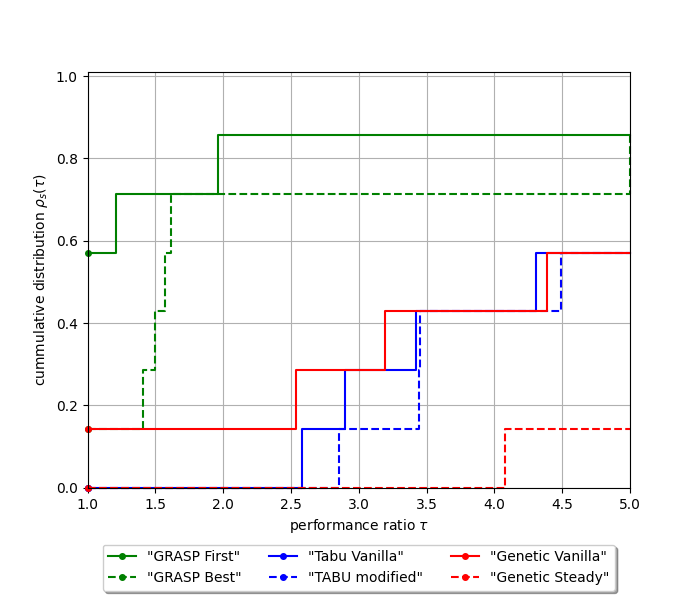
\includegraphics[width=\textwidth]{figure/performance_profile/performance_profile_thmax_5.0.png}
    \caption{Gráfico de \perfprof no intervalo $[1, 5]$}
    \label{fig:performance-profile-5}
\end{figure}

\begin{figure}[H]
    \centering
    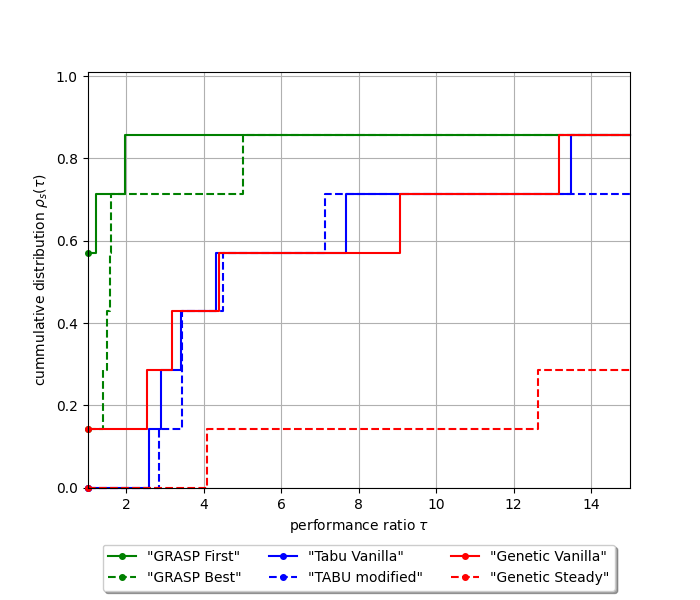
\includegraphics[width=\textwidth]{figure/performance_profile/performance_profile_thmax_15.0.png}
    \caption{Gráfico de \perfprof no intervalo $[1, 15]$}
    \label{fig:performance-profile-15}
\end{figure}

\begin{figure}[H]
    \centering
    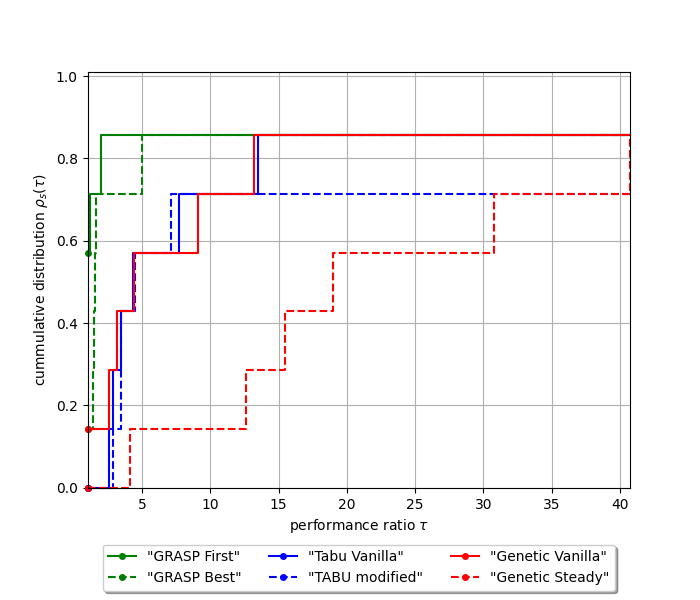
\includegraphics[width=\textwidth]{figure/performance_profile/performance_profile_thmax_None.png}
    \caption{Gráfico de \perfprof no intervalo $r_M$ (calculado automaticamente pelo software de plot).}
    \label{fig:performance-profile-max}
\end{figure}
